

%----------------------------------------------------------------------%
\section{Motiviation Web Scraping}
%----------------------------------------------------------------------%
\begin{frame}
\frametitle{Motiviation Web Scraping}



\begin{figure}[H] \centering
  \centering
  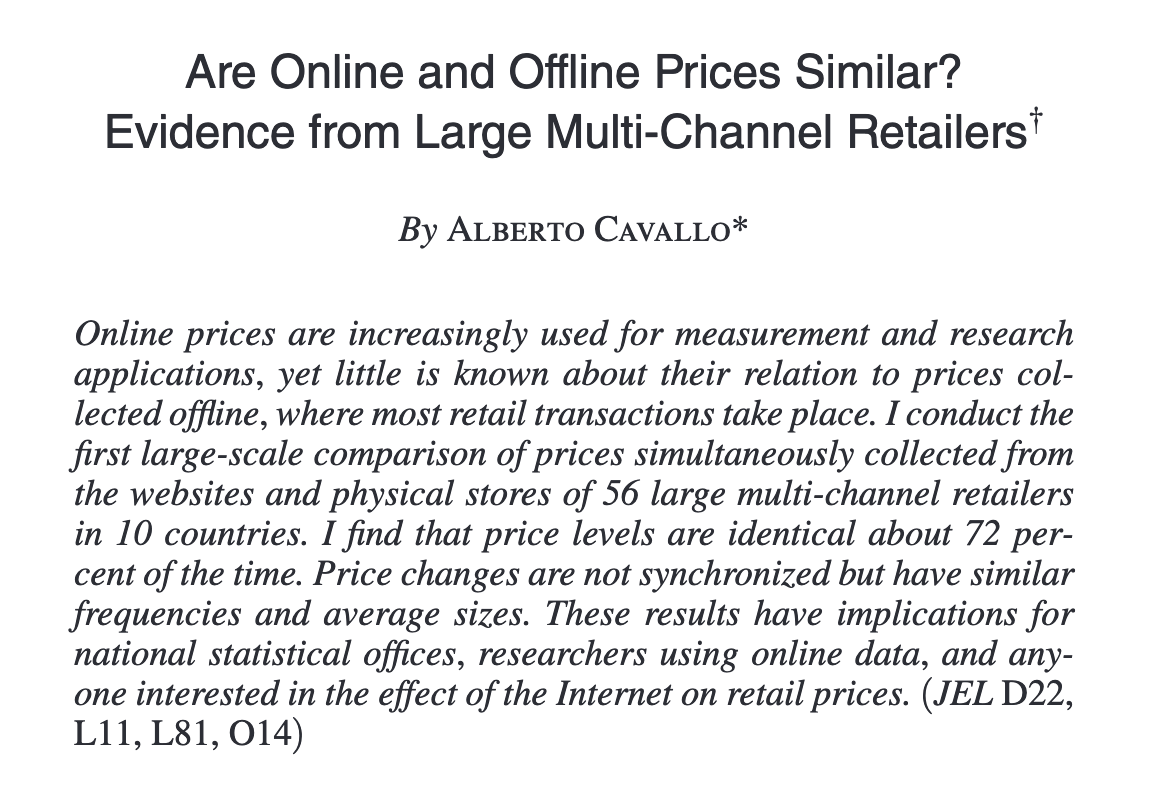
\includegraphics[scale=0.45]{figures/Cavallo_title}
  \\
  \tiny
\end{figure}
 

\end{frame}

%----------------------------------------------------------------------%
\begin{frame}
\frametitle{Motiviation Webscraping}



\begin{figure}[H] \centering
  \centering
  
\includegraphics[scale=0.25]{figures/Cunningham_title}
  \\
  \tiny
\end{figure}
 

\end{frame}

%----------------------------------------------------------------------%

\begin{frame}
\frametitle{Motiviation Webscraping}



\begin{figure}[H] \centering
  \centering
  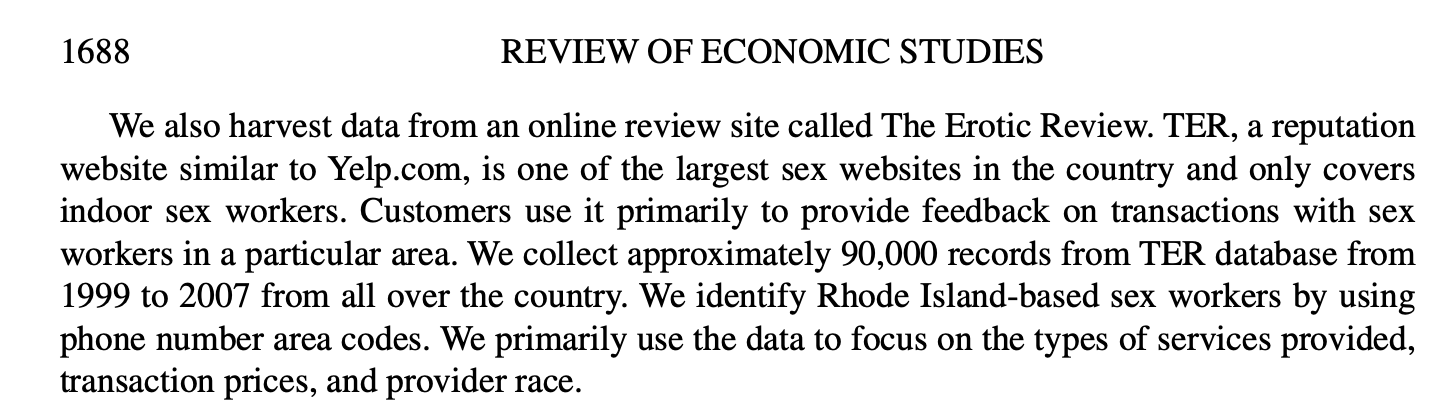
\includegraphics[scale=0.45]{figures/Cunningham_desc}
  \\
  \tiny
\end{figure}
 

\end{frame}


%----------------------------------------------------------------------%

\begin{frame}
\frametitle{Webscraping basics}

\begin{figure}[H] \centering
  \centering
  
\includegraphics[scale=0.75]{figures/webscrape_it.jpg}
  \\
  \tiny
\end{figure}

\end{frame}

%----------------------------------------------------------------------%
\begin{frame}
\frametitle{Webscraping basics}

\begin{itemize}
  \item How to get data, or "content", off the web and onto our computers.
  \bigskip
  \item If you see it in your browser it exists somewhere
  \bigskip
  \item To be ``successful'' one must have a working knowledge on:
  \begin{itemize}
  \item how web pages display content (Hyper Text Markup Language or HTML)
  \medskip
  \item where is the content ``located''


    \begin{enumerate}
    \item Server side
    \medskip
    \item Client side
    \medskip

    \end{enumerate}
    \item The good news is that both server-side and client-side websites allow for web scraping
   \end{itemize}
\end{itemize}





\end{frame}

%----------------------------------------------------------------------%
\begin{frame}
\frametitle{Caveat: ethical and legal limitations}

\begin{itemize}
\item Just because you *can* scrape it, doesn't mean you *should*. 
\medskip
\item Check \texttt{The Robots Exclusion Protocol} of a website, adding \texttt{``/robots.txt''} to the website's URL
\begin{enumerate}
  \item User-agent:  the type of robots to which the section applies
  \item Disallow:  directories/prefixes of the website not allowed to robots
  \item Allow:  sections of the website allowed to robots
\end{enumerate}
\medskip
\item \texttt{robots.txt} is de facto standard (see \url{http://www.robotstxt.org})
\medskip
\item Also always check the terms and conditions and what they say about scraping
\medskip
\item Remember the immortal words of uncle Ben: ``with great power comes great responsibility''

\end{itemize}


\end{frame}